\documentclass[12pt]{beamer}
\usepackage{beamerthemeHannover, graphicx, clrscode, amsmath, amssymb, multicol}
\usepackage{verbatim}
\setbeamercolor{sidebar}{use=structure,bg=gray!20!red!60!white}
\title{Getting Involved With Rakudo \\ \small{ (A Flavor of Perl 6) } }
\author[Duke Leto]{Jonathan "Duke" Leto}
\date{}

\begin{document}

\frame{
    \titlepage
    \begin{center}
        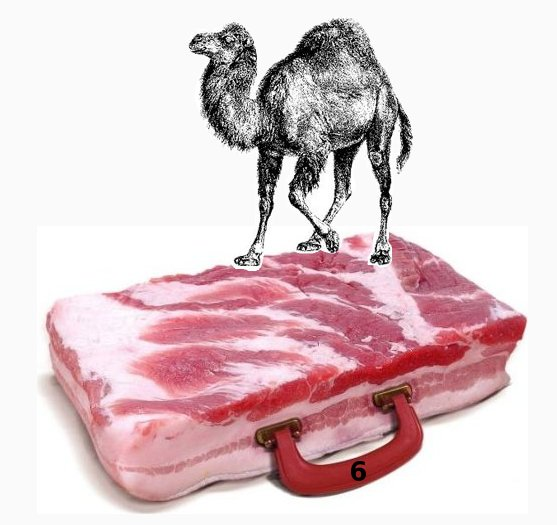
\includegraphics[width=4.57cm, height=4.25cm]{perl6bacon}
    \end{center}
}

\section{What is Perl 6?}
\frame{
    \frametitle{Flavors of Perl 6}
    \begin{center}
        \begin{itemize}
            \item Rakudo - Parrot
            \item Pugs - Haskell
            \item SMOP - C+DSLs
            \item Elf - Ruby
            \item STD.pm - Larry's Implementation in Perl 6 (gimme5)
            \item v6.pm - Source filter for Perl 5
            \item others ...
        \end{itemize}
    \end{center}
}

\frame{
    \frametitle{What is Rakudo?}
    \begin{center}
    \begin{quotation}
    The Way Of The Camel  = "Rakuda-do" $\implies$ Rakudo, which happens to mean "paradise" in Japanese.
    \end{quotation}

        \begin{itemize}
            \item Perl 6 implementation on the Parrot Virtual Machine
            \item Still lives in \begin{bf}languages/perl6\end{bf} directory of Parrot
            \item Fierce development in the last few weeks
            \item Aiming to be the first production Perl 6 implementation
            \item 1.0 ? Sometime before Xmas
        \end{itemize}
    \end{center}
}

\section{Getting Started}

\frame{

    \frametitle{Getting Involved}
    \begin{itemize}
        \item {\tiny{ http://trac.parrot.org/parrot/wiki/NewParrotDeveloperGuide } }
        \item Help finish porting the Wiki from SocialText to TracWiki on parrot.org
        \item Beginner tutorials are sorely needed
        \item Fix/contribute documentation
        \item Report bugs on your platform/set up a BuildBot slave
        \item Blog your Rakudo/Perl 6 experiences to combat FUD
    \end{itemize}
}
\frame{
    \frametitle{Can You Smell The Bacon?}
    \begin{columns}[t]
    \begin{column}[T]{8cm}
        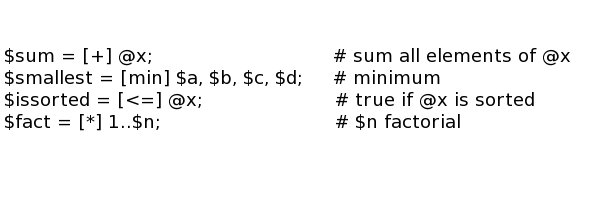
\includegraphics[width=6.00cm, height=2.00cm]{perl6code1} \\
        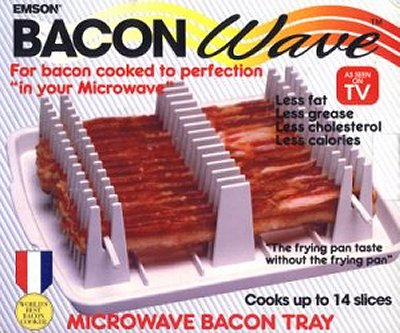
\includegraphics[width=4.00cm, height=4.00cm]{BaconWave}
    \begin{block}{PROTIP:}
        perldoc foo.pir
    \end{block}

    \end{column}
    \end{columns}

}

\section{ Let's Jump In }
\frame{
    \frametitle{Hack Session}
    Ok, let's do some hacking already.
    \begin{itemize}
        \item Checkout source code (svn co ... )
        \item Build parrot and perl6 (make perl6)
        \item Build docs (make html)
        \item Run tests for parrot and perl6
        \item Submit bugs if any tests fail
        \item Experiment!
    \end{itemize}
}

\frame{
    \frametitle{ Thanks }
    \begin{itemize}
        \item Larry
        \item Eric Wilhelm
        \item Jerry Gay
        \item Patrick Michaud
        \item The Perl Foundation
        \item Everyone working on Parrot, Rakudo and Perl 6
    \end{itemize}
}

\frame{
    \frametitle{ Resources }
    \begin{center}
        \begin{itemize}
           \item http://rakudo.org
           \item http://parrot.org
           \item http://perlsphere.net
           \item \#perl6 and \#parrot on freenode
           \item \#pdx.pm on irc.perl.org
        \end{itemize}
    \end{center}
}
\end{document}
